\chapter{Host Organization and Project Context}\label{ch:context}
\section*{Introduction}
Before diving into the technical work, it is important to understand the environment in which it was carried out --- who the host organization is, what they do, and why this project exists in the first place. This chapter covers exactly that. We start with an overview of Huawei as a company: its history, mission, and how it is structured internally. We then zoom into the Sales and Solutions Department, which hosted this internship, and the SmartCare platform that sits at the core of the project. From there, we shift to the project context itself --- the industry background, the technological factors at play, and the specific challenges that motivated the work. By the end of this chapter, the problem this project is solving 
should be clear, and the rest of the report can be read with that foundation in mind.

\section{Host Organization: Huawei}
\begin{figure}[htbp]
    \centering
    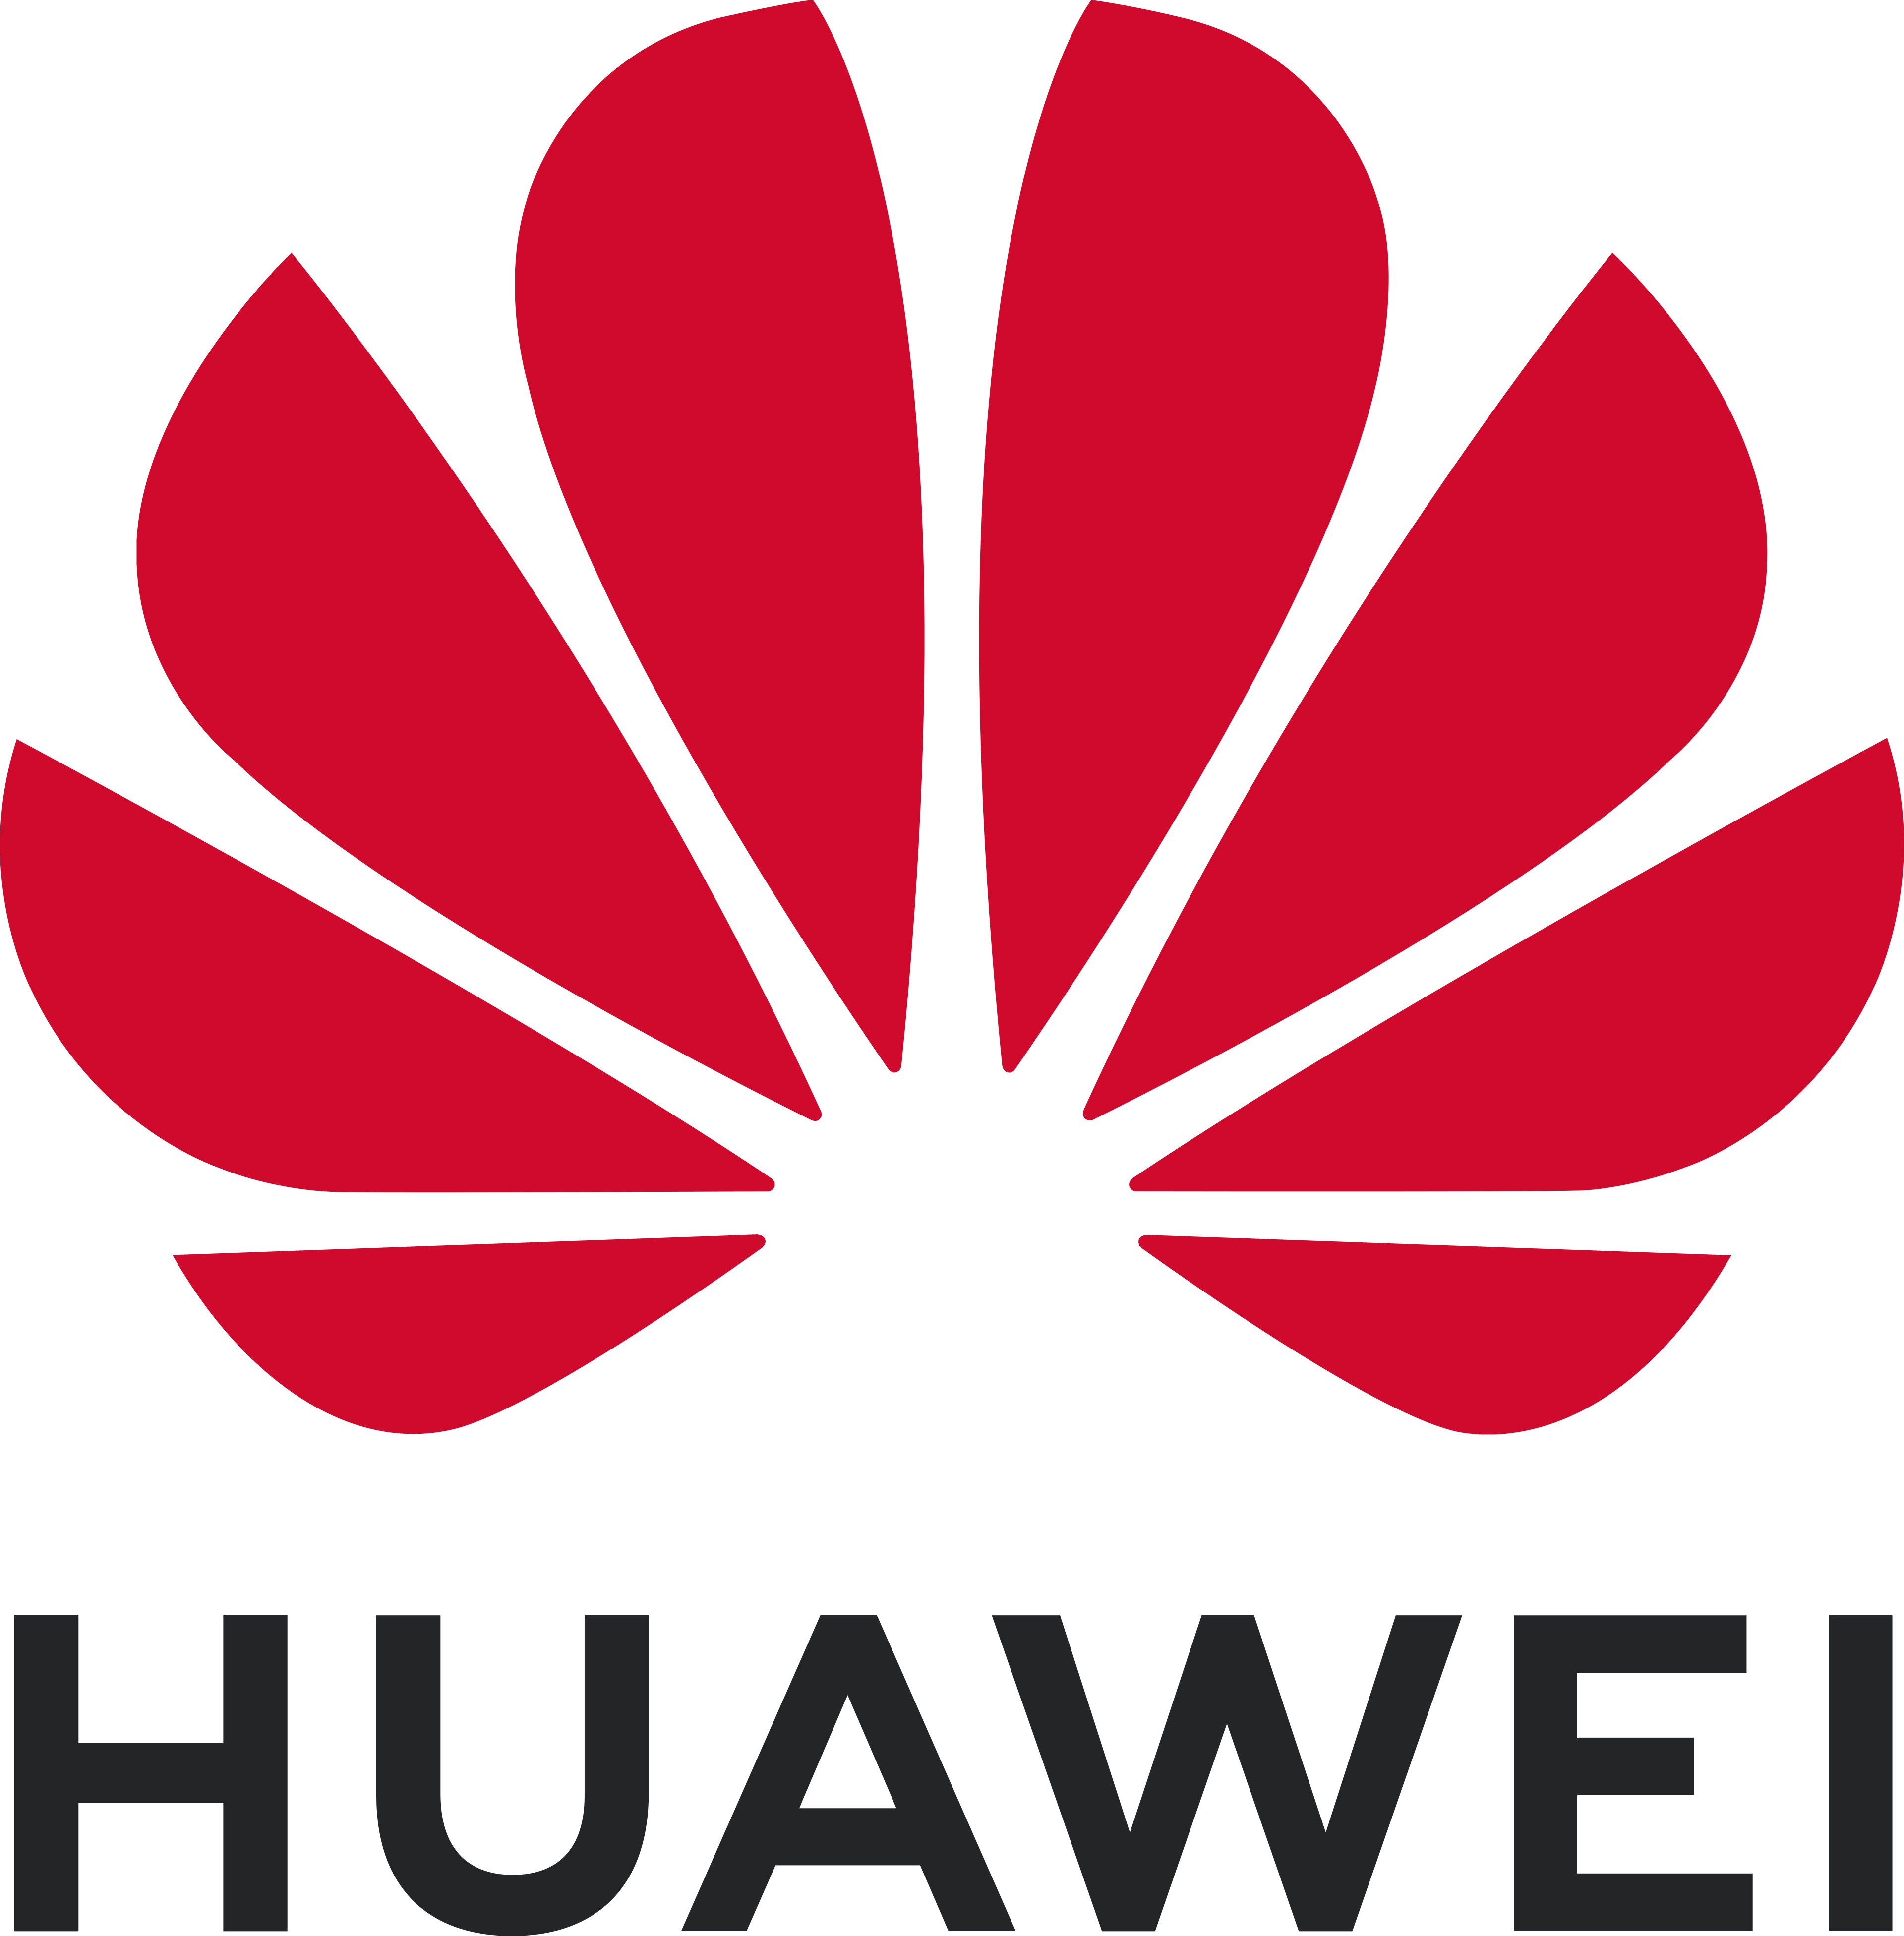
\includegraphics[width=0.2\textwidth]{figures/company_logo.png}
    \caption{Company Logo}
    \label{fig:company-logo}
\end{figure}

\subsection{Company Overview}
Founded in 1987 in Shenzhen, China, Huawei Technologies Co., Ltd. is a leading global 
provider of Information and Communications Technology (ICT) infrastructure and smart 
devices. With approximately 213,000 employees operating across more than 170 countries 
and regions, Huawei serves upwards of 3 billion people worldwide \cite{huawei_about}. 
Over nearly four decades, the company has evolved from a sales agent for Private Branch 
Exchange (PBX) switches into one of the world's largest technology corporations, 
sustaining this growth through a sustained commitment to research and development: in 
2025 alone, Huawei invested CNY~192.3 billion in R\&D, representing 21.8\% of its total 
revenue, with over 53\% of its workforce engaged in research activities \cite{huawei_about}.

Within its carrier-facing portfolio, Huawei offers a broad range of solutions to help 
Communication Service Providers (CSPs) operate and optimize their networks --- and among 
those, \textbf{HUAWEI SmartCare} is one of the flagship ones. To keep it simple, 
SmartCare is a Customer Experience Management (CEM) platform: it brings together network 
analytics, subscriber management, and service assurance all in one place 
\cite{huawei_smartcare_cem}. It was originally built as a Service Operations Center (SOC) 
solution, the idea being to stop operators from always playing catch-up with network 
issues and instead get ahead of them --- detecting degradation before it reaches the end 
user \cite{huawei_smartcare_soc}.

At its core, SmartCare works through a three-tier indicator framework --- Customer 
Experience Indicators (CEIs), Key Quality Indicators (KQIs), and Key Performance 
Indicators (KPIs) --- giving operators a per-service, per-user, per-location view of what 
is actually happening on the network. It also covers QoE monitoring, fault
diagnosis, NPS tracking, and self-care integration. Gartner lists it as a
Representative Vendor for CSP service and network assurance, and it is certified
under the TM Forum ODA component directory
\cite{huawei_gartner}\cite{huawei_tmforum}.

This internship builds on that foundation with a new use case for the Sales and
Solutions Department: a conversational AI layer powered by a Large Language Model
(LLM), plus a churn prediction module. That was the brief at the start; what the
churn side actually became, and why, is covered in Chapter~\ref{ch:eval}. The
goal is to let sales and solutions engineers query live subscriber and network
data in plain language and surface at-risk subscribers --- extending SmartCare
into pre-sales and account management, where it currently doesn't reach.

\subsection{Mission and Strategic Vision}

Huawei's guiding mission is to bring digital to every person, home, and organization 
for a fully connected, intelligent world. This mission is operationalized through the 
company's All Intelligence Strategy, unveiled in 2023, which places AI at the center 
of every business domain --- from network infrastructure to enterprise cloud services 
to consumer devices.

The company's strategic pillars as articulated in its 2025 commitments are:
\begin{itemize}
    \item \textbf{Laying the groundwork for All Intelligence} --- building the 
    foundational infrastructure for an AI-driven era across industries.
    \item \textbf{Strengthening innovation, openness, and collaboration} --- investing 
    in basic research while remaining open to ecosystem partnerships.
    \item \textbf{Succeeding through quality and prioritizing security} --- treating 
    quality as a precondition for customer trust and long-term competitiveness.
    \item \textbf{Building thriving ecosystems for a shared future} --- fostering 
    developer communities (Kunpeng, Ascend, HarmonyOS) and partner networks.
    \item \textbf{Promoting sustainable development through digital inclusion} --- 
    extending connectivity to underserved populations and reducing carbon footprints 
    through digital power solutions.
\end{itemize}

Quality occupies a central place in Huawei's corporate culture, formalized in its 
Quality Policy: ``Always keep in mind that quality is the foundation of Huawei's 
survival, and the reason for the customer to choose Huawei.''

\subsection{Organizational Structure}

Huawei runs on a \textbf{matrix organizational model} --- product-line specialization 
on one axis, regional customer proximity on the other. The company is structured around 
three primary Business Groups (BGs) and two dedicated Business Units (BUs), as shown 
in Table~\ref{tab:huawei_org}.

\begin{table}[h!]
\centering
\renewcommand{\arraystretch}{1.4}
\begin{tabular}{|p{5.5cm}|p{8.5cm}|}
\hline
\textbf{Division} & \textbf{Focus Area} \\
\hline
Carrier Business Group (Carrier BG) & Wireless networks, fixed networks, core networks, 
carrier software, and global services for telecommunications operators \\
\hline
Enterprise Business Group (Enterprise BG) & Data center infrastructure, storage, and 
digital transformation solutions for enterprises and industries \\
\hline
Consumer Business Group (Consumer BG) & Smartphones, PCs, tablets, wearables, HarmonyOS 
ecosystem, and intelligent driving solutions \\
\hline
Cloud \& AI BU & Cloud computing services, AI platforms (Pangu Models), and developer 
ecosystems (Kunpeng, Ascend) \\
\hline
Digital Power BU & Energy-efficient power solutions, green energy generation, and smart 
grid infrastructure \\
\hline
\end{tabular}
\caption{Huawei Business Groups and Units}
\label{tab:huawei_org}
\end{table}

\subsection{Regional and Sales Structure}

On the commercial side, operations are split across geographic regions, each under a 
Regional Sales Vice President who oversees the country-level offices below them. Day 
to day, it's a dual-track setup: \textbf{lead account teams} at headquarters keep an 
eye on the big accounts, while \textbf{local channel teams} and regional enterprise 
teams handle the actual delivery, customization, and partner work on the ground. 
Global product capabilities, local execution --- that's the idea.

This internship was carried out within the \textbf{Sales and Solutions Department}, 
sitting under the Carrier Business Group. The department's job is essentially to 
translate Huawei's technical portfolio into something a customer can act on --- 
proposals, demos, data-driven recommendations. SmartCare is one of the core platforms 
they present and sell, which is exactly what made it the right home for this project.

\section{Project Context}

\subsection{Background}

\subsubsection{Historical Context}

In the telecom and operator industry, the past three decades have brought profound 
structural change. Networks evolved from Circuit-Switched (CS) voice in 2G, to 
Packet-Switched (PS) architectures in 3G, through Long-Term Evolution (LTE) in 4G, 
and up to the current deployment of fifth-generation (5G) networks. This progression 
not only improved bandwidth and latency, but gave rise to an unprecedented volume of 
operational data --- KPIs, KQIs, network campaigns, and subscriber behavior records 
accumulating at a scale that traditional tooling was never designed to handle. 
Network hardware vendors such as Huawe, which delivered the world's first commercial LTE/EPC network 
in 2009 and has since supported the deployment of 5G as well, across more than 170 countries 
worldwide, have gathered expertise in managing this complex, multi-layered infrastructures. Yet 
the tools used to query, interpret and act upon the data they produce have historically been the 
drawback, relying on dashboards, manual reporting and siloed analyst workflows. SmartCare was built to 
help close that gap on the network ops side, but the sales layer wasn't really touched.

However this changed after the emergence of LLMs between 2020 and the present, a new frontier has opened:
the ability to query structured operational data in plain natural language, without SQL expertise 
or intimate knowledge of database schemas. But beyond just fetching data, an LLM can reason over the results, 
spot patterns and give a conclusion, helping a sales manager or solutions engineer to get to the 
right question faster, without relying on a data analyst on standby.
\subsubsection{Socioeconomic and Technological Factors}

Several converging factors shaped the environment in which this project was conceived. 
The commercial rollout of 5G introduced a new layer of network complexity, with 
operators now managing simultaneous multi-generation subscriber bases spanning 2G 
through 5G --- each with distinct usage profiles, churn behaviors, and upgrade 
trajectories. Migrating subscribers toward newer technologies therefore requires a 
strategic viewpoint and surgical precision when analyzing network variables, making 
data-driven tooling not just convenient but operationally necessary.

On the infrastructure side, while LLMs are inherently resource-intensive, a company 
of Huawei's scale can leverage cloud-hosted inference APIs, ensuring access to the 
latest high-reasoning models without the overhead of local hardware provisioning. 
That said, data privacy regulations and enterprise security requirements impose 
constraints on what data can be externalized to commercial services --- reinforcing 
the need for locally deployable or tightly controlled inference solutions as a 
complementary approach.

\subsubsection{Current Challenges}\label{sec:challenges}

Despite the availability of rich operational data --- and despite SmartCare already 
handling the network operations side --- several challenges persist when it comes to 
actually using that data in a sales and solutions context. Database schemas in 
telecom environments are large, relational, and non-trivial: even experienced 
analysts make errors constructing queries across multi-table subscriber and network 
datasets. Churn prediction, something carrier customers care a lot about, typically 
requires a purpose-built machine learning pipeline --- and those are rarely integrated 
with the conversational or dashboard tools sales teams actually use. On top of that, 
the time between a business question coming up in a customer meeting and getting a 
data-backed answer is still too long, which limits how agile a solutions engagement 
can be.

These gaps --- raw data vs.\ actionable insight, ML outputs vs.\ operational 
dashboards, natural language questions vs.\ structured query results --- are exactly 
what this project is trying to close, by bringing that capability into SmartCare's 
ecosystem.

\bigskip
\noindent The following section defines the specific problem statement this project 
was designed to solve, drawing directly from the operational context described above.
\section{Conclusion}
In this chapter, we introduced Huawei as the host organization --- its history, structure, and the SmartCare platform that sits at the center of this project. We also laid out the context that motivated the work: a telecom industry generating more operational data than existing tools can handle, and a sales layer that still largely relies on manual effort to make sense of it. The following chapters get into the actual work --- starting with the system architecture and the data foundation we built to support it.
